% LaTeX Präsentationsvorlage (2013) der TU Graz, rev12, 2013/01/31
\documentclass{beamer}
% \documentclass[aspectratio=169]{beamer}
\usetheme{tugraz2013}
% \usetheme[notes]{tugraz2013}
% \usetheme[minimal]{tugraz2013}

%% Titelblatt-Einstellungen
\title[Waterbot]{Waterbot}%%:\\Exploring Feedback and \\Persuasive Techniques at the Sink}
\author{Robert Thomann, Manuel Zoderer}
\date{Graz, 23. March 2015}		% \today für heutiges Datum verwenden
%\date{\today}
%%\institute[]{}
\instituteurl{www.tugraz.at}
% \institutelogo{kurz.pdf}
% \additionallogo{institutslogo.pdf}

%%%%%%%%%%%%%%%%%%%%%%%%%%%%%%%%%%%%%%%%%%%%%%%%%%%%%%%%%%%%%%%%%%%%%%%%%%%%
\begin{document}
%%%%%%%%%%%%%%%%%%%%%%%%%%%%%%%%%%%%%%%%%%%%%%%%%%%%%%%%%%%%%%%%%%%%%%%%%%%%
\titleframe

\begin{frame}
  \frametitle{The Paper}
  \begin{quote}``Waterbot: Exploring Feedback and Persuasive Techniques at the Sink''\end{quote}
  \begin{itemize}
  \item Authors: 
    \begin{itemize} 
    \item Ernesto Arroyo
    \item Leonardo Bonanni
    \item Ted Selker
    \end{itemize}
  \item MIT Media Laboratory
  \end{itemize}
\end{frame}


\begin{frame}
  \frametitle{Content}
  \tableofcontents%[hideallsubsections] 
\end{frame}


%%%%%%%%%%%%%%%%%%%%%%%%%%%%%%%%%%%%%%%%%%%%%%%%%%%%%%%%%%%%
\section{Overview}

\begin{frame}
	\frametitle{Overview}
	\begin{itemize}
	  \item A system to inform and motivate behavior at the sink
          \item Persuasive techniques (instead of automatisation)
          \item Four prototypes
	    \begin{itemize}
              \item HeatSink
              \item SeeSink
              \item CleanSink
              \item WaterBot
            \end{itemize}          
        \end{itemize}          

\end{frame}


\begin{frame}
  \frametitle{HeatSink}

  \begin{columns}[c] % the "c" option specifies center vertical alignment
    \column{.5\textwidth} % column designated by a command
    Iluminates the water stream dependent on its temperature
    \column{0.5\textwidth}
    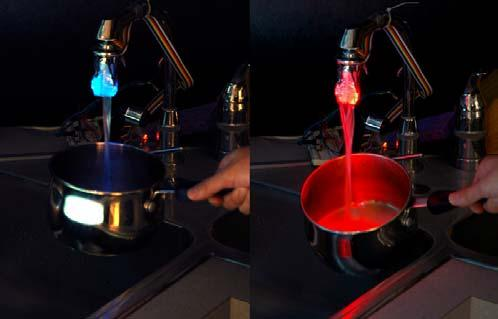
\includegraphics[width=\textwidth]{Bilder/HeatSink.jpg}
  \end{columns}
\end{frame}


\begin{frame}
  \frametitle{SeeSink}
  \begin{columns}[c]
    \column{.5\textwidth}
    \begin{itemize}
    \item tasks detected with CCD camera
    \item automatic temperature and flow control
    \item ilumination like HeatSink
    \end{itemize}
    \column{0.5\textwidth}
    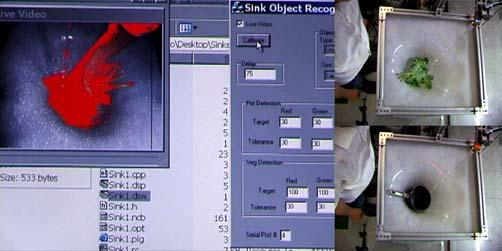
\includegraphics[width=\textwidth]{Bilder/SeeSink.jpg}
  \end{columns}

\end{frame}


\begin{frame}
  \frametitle{CleanSink}
  For monitoring of hand-washing compliance.
  \begin{columns}[c]
    \column{.5\textwidth}
    \begin{itemize}
    \item flashing after time
    \item RFID login
    \item connected with environment\\(lights, locks)
    \end{itemize}
    \column{0.5\textwidth}
    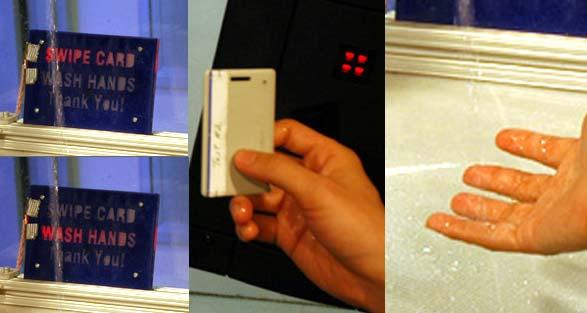
\includegraphics[width=\textwidth]{Bilder/CleanSink.jpg}
  \end{columns}

\end{frame}


\begin{frame}
  \frametitle{WaterBot}
  \begin{columns}[c]
    \column{.5\textwidth}
    \begin{itemize}
    \item tracks water usage
      \begin{itemize}
      \item time
      \item flow
      \end{itemize}
    \item visual feedback
      \begin{itemize}
      \item HeatSink
      \item LED bars
      \end{itemize}
    \item auditory messages
    \end{itemize}
    \column{0.5\textwidth}
    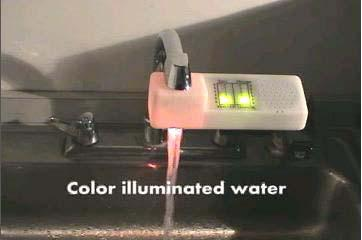
\includegraphics[width=\textwidth]{Bilder/WaterBot.jpg}
  \end{columns}


\end{frame}








%%%%%%%%%%%%%%%%%%%%%%%%%%%%%%%%%%%%%%%%%%%%%%%%%%%%%%%%%%%%
\section{Motivation}
\begin{frame}
	\frametitle{Motivation}
	\begin{itemize}
	  \item Test HCI in hostile environment
	  \item Test persuasive techniques
          \item Test different feedback approaches
        \end{itemize}          

\end{frame}

%%%%%%%%%%%%%%%%%%%%%%%%%%%%%%%%%%%%%%%%%%%%%%%%%%%%%%%%%%%%
\section{Insights}
\begin{frame}
	\frametitle{Insights}
	\begin{itemize}
	  \item HCI can work in environmentally challenging places.
          \item Automation can be replaced by persuasive techniques.
          \item Some feedback approaches are better recieved than others.
        \end{itemize}          

\end{frame}
%%%%%%%%%%%%%%%%%%%%%%%%%%%%%%%%%%%%%%%%%%%%%%%%%%%%%%%%%%%%
\section{Methodology}
\begin{frame}
	\frametitle{Methodology}
	\begin{itemize}
	  \item Seven design principles identified
	  \item Pilot study: 10 users
          \item User study: 2 months, 15 users, community sink
        \end{itemize}          

\end{frame}

\begin{frame}
	\frametitle{Methodology - Shortcommings}
	\begin{itemize}
	  \item Some data is not included.
	  \item Lack of structure in user study.
        \end{itemize}          


\end{frame}


%%%%%%%%%%%%%%%%%%%%%%%%%%%%%%%%%%%%%%%%%%%%%%%%%%%%%%%%%%%%
\section{Impact}
\begin{frame}
	\frametitle{Impact}
        Practical applications:
	\begin{itemize}
	  \item improve safety
          \item improve hygiene
          \item conserve water
        \end{itemize} 
        Possible foundation for future studies.
\end{frame}

\begin{frame}
	%\frametitle{Impact 2}
        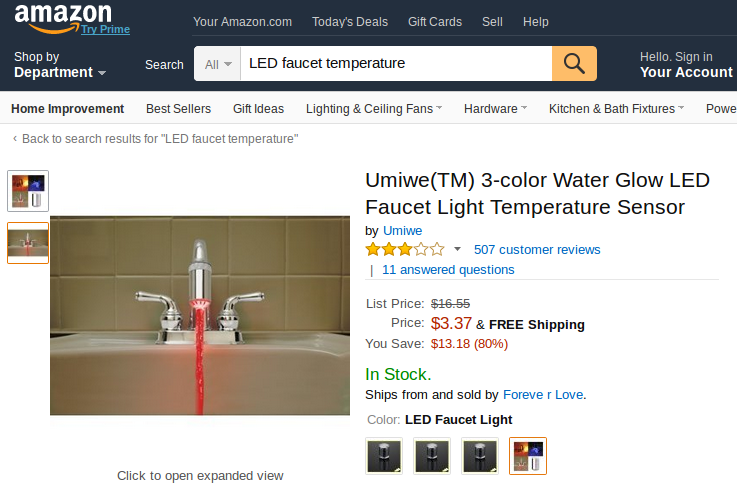
\includegraphics[width=\textwidth]{Bilder/faucet1.png}
        
\end{frame}




%%%%%%%%%%%%%%%%%%%%%%%%%%%%%%%%%%%%%%%%%%%%%%%%%%%%%%%%%%%%%%%%%%%%%%%%%%%%
%%% Start Template
%%%%%%%%%%%%%%%%%%%%%%%%%%%%%%%%%%%%%%%%%%%%%%%%%%%%%%%%%%%%%%%%%%%%%%%%%%%%

%% \section{Einleitung}
%% \begin{frame}
%% 	\frametitle{Ziele der ersten Vorlesung}
%% 	Einführung in die KORE
%% 	\begin{itemize}
%% 		\item Geschichte der KORE kennen lernen
%% 		\item Aufgaben der KORE und Einordnung in das betriebliche Rechnungswesen verstehen
%% 		\item Wertebenen im Rechnungswesen unterscheiden
%% 	\end{itemize}
	
%% 	Grundlagen der KORE
%% 	\begin{itemize}
%% 		\item Kostenwürfel als Hilfsmittel verwenden
%% 		\item Überleitung von externem zu internem Rechnungswesen durchführen
%% 	\end{itemize}
%% \end{frame}

%% \begin{frame}
%% 	\frametitle{Titel der Folie\\maximal zwei Zeilen}
%% 	Text Ebene 1
%% 	\begin{itemize}
%% 		\item Zweite Ebene
%% 		\begin{itemize}
%% 			\item Dritte Ebene
%% 			\begin{itemize}
%% 				\item Vierte Ebene
%% 			\end{itemize}
%% 		\end{itemize}
%% 	\end{itemize}
%% \end{frame}

%% %%%%%%%%%%%%%%%%%%%%%%%%%%%%%%%%%%%%%%%%%%%%%%%%%%%%%%%%%%%%%%%%%%%%%%%%%%%%
%% \section{Aufzählungen}
%% %%%%%%%%%%%%%%%%%%%%%%%%%%%%%%%%%%%%%%%%%%%%%%%%%%%%%%%%%%%%%%%%%%%%%%%%%%%%

%% \section{Formeln und Links}
%% \begin{frame}
%% 	\frametitle{Formeln und Links}
%% 	Eine Formel:
%% 	\begin{eqnarray*}
%% 	u(x,t) & = & \sum_{k=1}^{\infty} f_k \sin \frac{k \pi x}{L} \cos 
%% 				 \frac{k \pi t}{aL} + \\
%% 		   & + & \sum_{k=1}^{\infty} g_k \sin \frac{k \pi x}{L} \sin 
%% 				 \frac{k \pi t}{aL} \\
%% 	\end{eqnarray*}

%% 	Ein Link:
%% 	\begin{center}
%% 		\url{http://www.tugraz.at}		
%% 	\end{center}
%% \end{frame}

%% %%%%%%%%%%%%%%%%%%%%%%%%%%%%%%%%%%%%%%%%%%%%%%%%%%%%%%%%%%%%%%%%%%%%%%%%%%%%
%% \section{Quelltexte}
%% \begin{frame}[fragile]
%% 	\frametitle{Quelltexte}
%% 	\begin{spacing}{1}
%% 	\begin{semiverbatim}
%% SUCHE (A,x)
%% 1: i = 0
%% 2: WHILE i<n
%% 3:     i = i+1
%% 4:     \alert{IF A[i]=x THEN RETURN i}
%% 5: ELSE RETURN -1
%% 	\end{semiverbatim}
%% 	\end{spacing}
%% \end{frame}

%% %%%%%%%%%%%%%%%%%%%%%%%%%%%%%%%%%%%%%%%%%%%%%%%%%%%%%%%%%%%%%%%%%%%%%%%%%%%%

%% \section{Spalten und Grafiken}
%% \begin{frame}
%% 	\frametitle{Zwei Inhalte Links/Rechts\\Wahlweise Text/Grafik}
%% 	\begin{columns}[onlytextwidth]
%% 		\begin{column}{0.5\textwidth}
%% 			\begin{itemize}
%% 				\item Lorem ipsum dolor sit amet, consectetur 
%% 				\item adipisicing elit, sed do eiusmod tempor 
%% 				\item incididunt ut labore et dolore magna aliqua. 
%% 				\item Ut enim ad minim veniam, quis nostrud 
%% 			\end{itemize}
%% 		\end{column}
%% 		\begin{column}{0.5\textwidth}
%% 			\begin{center}
%% 			
\includegraphics[width=0.5\textwidth]{logo.pdf}\\
%% 			Grafik in Spalte 2
%% 			\end{center}
%% 		\end{column}
%% 	\end{columns}
%% \end{frame}

%% \section{Weitere Beispielfolien}

%% \begin{frame}
%% 	\frametitle{Nur Titel \\maximal 2-zeilig}
%% \end{frame}

%% \sectionheader[Untertitel]{Abschnittsbeginn}

%% %%%%%%%%%%%%%%%%%%%%%%%%%%%%%%%%%%%%%%%%%%%%%%%%%%%%%%%%%%%%%%%%%%%%%%%%%%%%
%% \section{Zusammenfassung}
%% %%%%%%%%%%%%%%%%%%/%%%%%%%%%%%%%%%%%%%%%%%%%%%%%%%%%%%%%%%%%%%%%%%%%%%%%%%%%%

%% \begin{frame}
%% 	\frametitle{Zusammenfassung}
%% 	\begin{itemize}
%% 		\item Punkt 1
%% 		\item Punkt 2
%% 		\item Punkt 3
%% 	\end{itemize}
%% \end{frame}

%%%%%%%%%%%%%%%%%%%%%%%%%%%%%%%%%%%%%%%%%%%%%%%%%%%%%%%%%%%%%%%%%%%%%%%%%%%%
\end{document}
%%%%%%%%%%%%%%%%%%%%%%%%%%%%%%%%%%%%%%%%%%%%%%%%%%%%%%%%%%%%%%%%%%%%%%%%%%%%

%% EOF
